\chapter{Propuesta}\label{chapter:proposal}

\section{Captura de señales}
	Las señales que se consideraron capturar son las proporcionadas por sensores como el \textbf{acelerómetro},
	el \textbf{giroscopio} y el \textbf{GPS}, pues son los sensores más comunes en los teléfonos inteligentes. El
	\textbf{acelerómetro} como se explica en la literatura permite medir en tiempo real la aceleración(rapidez de
	cambio de la \textbf{velocidad}) en $m/s^2$ con respecto a los 3 ejes principales, y en el caso de los
	acelerómetros integrados en los teléfonos inteligentes permite medir la aceleración en los 3 ejes
	principales del dispositivo en cuestión. Estos 3 ejes se encuentran ubicados, si se sostiene el
	dispositivo de la forma usual, de la siguiente manera:

	\begin{itemize}
		\item eje X: Va de un lado del dispositivo a otro.
		\item eje Y: Va desde la parte inferior hasta la parte superior del dispositivo.
		\item eje Z: Es ortogonal a la pantalla del dispositivo.
	\end{itemize}
	
	\begin{figure}[htb]
		\centering
		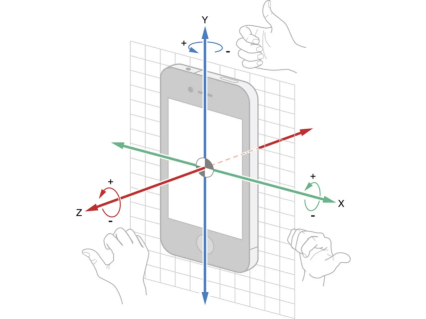
\includegraphics[scale = 0.5]{Graphics/mobile_phone_axis.png}
		\caption{Ejes de un dispositivo móvil}
		\label{fig:1}
	\end{figure}

	\subsection{Acelerómetro}
		La señal del \textbf{acelerómetro} mientras el vehículo se desplaza por carreteras en buen estado es bien similar,
		sin embargo una vez pasa por encima de un bache ocurre un evento anómalo en el que el vehículo se ve afectado
		por el bache, cayendo brevemente e incluso inclinándose momentáneamente hacia un lado (en el caso de un bache
		que afecte una sola rueda), por tanto la señal del \textbf{acelerómetro} en un intervalo de tiempo determinado debe tener
		un comportamiento fuera de lo común que permita identificar el evento en la serie temporal capturada por este sensor.
		Tal como se plantea en el estado del arte la característica fundamental de un bache son lecturas anormales en el eje
		Z del \textbf{acelerómetro} durante un intervalo de tiempo determinado, también dicho sensor debe registrar lecturas
		anormales en el eje X si el bache afecta un solo lado del vehículo, pues en este caso el vehículo se inclina violentamente
		hacia un lado por un momento.\\

	\begin{figure}[htb]
		\centering
		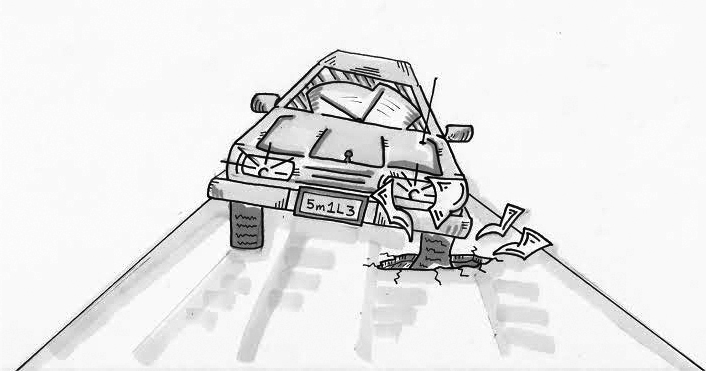
\includegraphics[scale = 0.5]{Graphics/one_side_pothole_vehicle.jpg}
		\caption{Vehículo impactado por un bache en un solo lado}
		\label{fig:2}
	\end{figure}

	\subsection{Giroscopio}
		El \textbf{giroscopio} es otro de los sensores que se considera aportaría información útil, ya que este sensor 
		mide en $rad/s$ la velocidad angular del dispositivo móvil con respecto a los 3 ejes mencionados previamente. 
		En el momento que un vehículo interactúa con un bache ocurren vibraciones que hacen que el vehículo gire, lo que
		debería generar picos en las lecturas del \textbf{giroscopio} en un intervalo de tiempo. El problema con este sensor es 
		que a pesar de ser de los más comunes, no es abundante en teléfonos inteligentes de gama baja por lo que 
		su uso en la propuesta de solución se tiene pensado como algo que permita mejorarla y no algo de lo que esta
		dependa.\\

	\subsection{GPS}
		El \textbf{GPS}(\emph{Global Positioning System}) es el sensor que le permite al dispositivo móvil ubicarse sobre la
		superficie de la tierra utilizando coordenadas de latitud-longitud. Debido a que este sistema utiliza señales para
		comunicarse con satélites en tiempo real, existe una latencia debido al tiempo que le toma a la señal viajar hacia el
		satélite y de vuelta al dispositivo. Además, las condiciones atmosféricas pueden afectar esta latencia, así como el hecho
		de que la señal puede ser reflejada por el terreno, edificios, etc., como por ejemplo cuando se viaja a través de un
		túnel subterráneo donde la señal no puede llegar. También es importante destacar que las lecturas que genera el \textbf
		{GPS} tienen cierto margen de error que varía de un dispositivo a otro y que depende de la potencia del sensor en sí,
		pero en general según la literatura la mediana del error en estos sensores es de 5m aproximadamente \parencite{eriksson2008pothole},
		ambos aspectos son importantes a tener en cuenta al hacer uso de este sensor. El mismo se puede utilizar para estimar la
		\textbf{velocidad} a la que viaja el vehículo, lo que es necesario ya que la \textbf{velocidad} es un factor que influye de
		forma directa en la forma que un vehículo es afectado por un bache, además con este sensor es posible ubicar en un mapa
		aproximadamente los lugares donde existen baches u otro tipo de anomalías, incluso puede ser útil para marcar rutas de viaje
		y así facilitar algunos aspectos de la propuesta de solución.

	\subsection{Velocidad y frecuencia de muestreo}
		La frecuencia de muestreo se tomó de tal forma que se tuviera una lectura de \textbf{acelerómetro} y \textbf
		{giroscopio} por cada metro. Si se va a una \textbf{velocidad} $v$ en $m/s$ y se quiere obtener $x$ muestras
		por cada metro, quiere decir que se necesitan obtener $v * x$ muestras, por lo que la frecuencia de muestreo
		necesaria sería de $\frac{1}{v * x} Hz$. Como se quiere una sola muestra por cada metro la frecuencia de muestreo
		en este caso particular es de $\frac{1}{v} Hz$. Debido a que la \textbf{velocidad} de un vehículo durante un
		recorrido no suele ser constante, es necesario que la \textbf{frecuencia de muestreo} cambie en función de la
		\textbf{velocidad} a la que vaya el vehículo, pues mientras más rápido vaya es necesario realizar más capturas
		con los sensores para no perder información importante. Este cambio de \textbf{frecuencia de muestreo} se propuso
		realizarlo cada 5 segundos.\\
		Para actualizar de forma correcta la \textbf{frecuencia de muestreo} es necesario conocer la \textbf{velocidad}
		a la que viaja el vehículo, o al menos realizar una estimación aceptable de la misma utilizando los sensores de
		los que dispone el dispositivo móvil. Esta estimación se realizó utilizando las lecturas del \textbf{GPS}, y se 
		asignaron frecuencias de muestreo teniendo en cuenta los límites de velocidad existentes en la zona urbana donde 
		se llevaron a cabo los experimentos. Debido a que en Cuba existen muy pocas carreteras donde se permita a
		los vehículos desplazarse a más de 100 km/h y también debido a que la mayoría de los vehículos que circulan en
		el país no alcanzan dicha \textbf{velocidad}, se asumió que esta es la máxima a la que podría desplazarse un
		vehículo a la hora de decidir las frecuencias de muestreo de los sensores.\\

	\subsection{Posición del móvil en el vehículo}
		La posición en la que se coloca el dispositivo móvil en el vehículo es relevante, al menos por ahora, pues la
		dirección del eje Y del vehículo debe coincidir con la del eje Y del móvil para que las señales que se capturen
		se correspondan con la realidad, de lo contrario se deberían realizar ciertos ajustes utilizando algún método de
		transformación de coordenadas para poder obtener lecturas acertadas sin importar la posición en la que se coloque
		el dispositivo.

\section{Detección de outliers}
	Los baches en la carretera no son más que anomalías como ya se mencionó. Teniendo en cuenta esto y ya con los \emph
	{datasets} al alcance, el primer paso fue identificar estas lecturas anómalas utilizando algún método de detección de \emph
	{outliers}(o \emph{novelty detection}). Para esto se probaron 2 vías:\\

	\begin{itemize}
		\item Se utilizaron 3 de los métodos heurísticos sugeridos en la literatura que pueden ser indicadores de la presencia de una
			anomalía en la carretera \textbf{Z-THRESH}, \textbf{Z-DIFF}, \textbf{G-ZERO}, que solamente necesitan los valores
			del \textbf{acelerómetro} en los 3 ejes.
		\item Se utilizaron algoritmos conocidos de \emph{Machine Learning} para detectar \emph{outliers} como \textbf{DBSCAN},
			\textbf{OPTICS} y \textbf{One Class SVM} con todos los features (no solo las lecturas del \textbf{acelerómetro}).
	\end{itemize}

	El proceso de detección con las heurísticas es sencillo, simplemente si algún valor excede los \emph{thresholds} establecidos en 
	cada método este se considera un \emph{outlier}. Para el proceso de detección de outliers con los algoritmos de aprendizaje no-supervisado
	se probaron 2 vías: 

	\begin{itemize}
		\item Detectar los \emph{outliers} en toda la serie temporal.\\
		\item Construir varias ventanas de cierto tamaño utilizando una ventana deslizante, extraer varios \emph{features} de
			cada una de estas ventanas y así generar nuevos \emph {features} para cada uno de los datos con el objetivo de
			intentar mejorar el proceso de detección de estos \emph{outliers}.\\
	\end{itemize}
	
	%Hablar sobre los hiperparámetros seleccionadas para cada uno de los métodos.

\section{Clasificación de outliers}

	%------------------------- Detallar que framework utilizamos para capturar los sensores ---------------------------
	% Primero que todo era necesario tener alguna forma de obtener señales de los sensores necesarios
	% para poder llevar a cabo nuestra propuesta. Para esto se apredió a trabajar en \textbf{Flutter} y
	% se hizo una aplicación móvil sencilla utilizando algunas bibliotecas propias de ese
	% \emph{framework} que nos permitiera obtener las señales de los sensores y exportarlas en un
	% {\textbf .json} para luego poder trabajar con dichos datos en el modelo de \emph{Machine Learning}.

